\documentclass[twocolumn]{aastex61}
\usepackage{bm}
\usepackage{color}
\usepackage{graphicx}
\usepackage{amsmath,amssymb}

\newcommand\teff{T_{\rm eff}}
\newcommand\logg{\log{g}}
\newcommand\feh{[\rm{Fe}/\rm{H}]}
\newcommand\labels{\mathcal{\ell}}
\newcommand\latents{\mathrm{X}}
\newcommand{\Dvector}[1]{\boldsymbol{#1}}
\newcommand{\veclabels}{\Dvector{\labels}}
\newcommand{\veclatents}{\Dvector{\latents}}
\newcommand{\vectheta}{\Dvector{\theta}}
\newcommand{\vecmu}{\Dvector{\mu}}
\newcommand{\vecsigma}{\Dvector{\sigma}}
\newcommand{\scale}{s}
\newcommand{\vecscale}{\Dvector{\scale}}

\newcommand{\project}[1]{\textsl{#1}}
\newcommand{\package}[1]{\texttt{#1}}
\newcommand{\acronym}[1]{{\small{#1}}}
\newcommand{\todo}[1]{\textcolor{red}{#1}}


\received{2018 XX XX}
\revised{2018 XX XX}
\accepted{2018 XX XX}

\graphicspath{figures/}

\submitjournal{AAS Journals}

\shorttitle{Short title}
\shortauthors{Hinkel et al.}

\begin{document}

\title{Long title}

\correspondingauthor{Natalie Hinkel}
\email{natalie.hinkel@gmail.com}

\author[0000-0003-0595-5132]{Natalie Hinkel}
\affiliation{Department of Physics \& Astronomy, 
			 Vanderbilt University, 
			 Nashville, TN 37235, USA}

\author[0000-0003-2866-9403]{David W. Hogg}
\affiliation{Center for Cosmology and Particle Physics, Department of Physics, 
			 New York University, 
			 726 Broadway, New York, NY 10003, USA}
\affiliation{Center for Data Science, 
			 New York University, 
			 60 Fifth Ave, New York, NY 10011, USA}
\affiliation{Max-Planck-Institut f\"ur Astronomie, 
			 K\"onigstuhl 17, D-69117 Heidelberg}
\affiliation{Flatiron Institute, 
			 162 Fifth Ave, New York, NY 10010, USA}

\author[0000-0003-0174-0564]{Andrew R. Casey}
\affiliation{School of Physics \& Astronomy, 
			 Monash University, 
			 Wellington Road, Clayton 3800, Victoria, Australia}
\affiliation{Faculty of Information Technology, 
			 Monash University, 
			 Wellington Road, Clayton 3800, Victoria, Australia}


\begin{abstract}
Abstract.
\end{abstract}


\keywords{}

\section{Introduction}
\label{sec:introduction}


\section{Data}
\label{sec:data}

There are $N$ stars and $M$ surveys that report up to a $D$-dimensional vector of
labels $\labels_{nm}$ for each star. Not all surveys report labels for all stars,
and the labels reported by each survey are incomplete, in that there will be an
incomplete set of labels for the $n$-th star from the $m$-th survey. For example,
some surveys may not report some chemical abundance labels for an element if that
element does not have electronic transitions present in the spectra. There are
labels that are omitted for other reasons.


\section{Methods}
\label{sec:methods}

We make the following assumptions:

\begin{itemize}
  \item We assume that stars have true properties that are hidden (latent) and
	 	not directly observable.
  \item The effective temperature $\teff$, surface gravity $\logg$, and detailed
  	    chemical composition (e.g., [Fe/H], [Si/H], et cetera) are among the set
	    of latent properties of a star that cannot be directly observed, but can 
	    be estimated given a stellar spectrum and a model that describes that 
	    spectrum. Here we refer to the estimates of the true latent properties
	    as labels.
  \item For the purposes of this work we will assume that there are up to $D$
  	    labels that are reported by $M$ surveys, for up to $N$ stars.
  \item We assume that the overlap of stars between those surveys is not complete.
  		There are stars that will not have estimated labels; some will be missing.
  \item We further assume that the reported labels will be incomplete for some
	    stars and surveys. A survey may report a chemical abundance label for 
	    most stars, but not all, and other surveys may not report any labels for
	    the same chemical element.
  \item We assume that the labels reported by a survey will systematically differ
  		from the true latent values due to model complexities, the availability 
		of atomic and molecular transitions given some spectral region, decisions 
		about which atomic and molecular transitions to model, or numerous other
		model decisions that differ between surveys.
  \item For the same reasons, we assume that the labels reported by different
  	    surveys will differ systematically with respect to each other.
  \item We assume that the systematic differences from the latent values to the
  		reported labels can be reasonably modelled by an affine transformation
		from the latent space to the label space.
  \item We assume that each survey will have a different affine transformation 
  		from latent space to the label space.
  \item We assume that each survey has some systematic error in the reported
  		labels, and that systematic error dominates over the random error for
		all stars and all labels.
  \item We assume that the systematic error for a given survey can be represented
        as a $D$-dimensional vector. That is to say that we assume that the systematic
        errors in label space are uncorrelated.
  \item We assume that the reported labels are the affine-transformed expectation 
  		value of a normal distribution. In other words, we assume gaussian errors
		on the reported labels. 
  \item We assume that the true latent variables are drawn from a normal distribution
  		with zero mean and unit variance, and that these quantities become
		interpretable by applying a scale $\scale$ and a mean offset $\mu$ in each
		$D$-dimension. \todo{For this work we simply fix the offset and scale based
		on the mean and standard deviation of the reported labels.}
  \item We assume that the latent variables are statistically independent in that
	    the true latent value of any one star is independent of all other stars.
\end{itemize}

Conditioned on these assumptions, the model we adopt is a latent variable model
where the reported labels $\labels_{nm}$ for the $n$-th star are drawn from a normal
distribution with a mean that is the product of the latent variables $\textrm{X}_{n}$
and the transformation matrix from the $m$-th survey. Without loss of generality this
model can be described as
\begin{eqnarray}
	\veclabels_{nm} & \sim & \mathcal{N}\left(\veclatents_{n}\cdot\vectheta_{m} + \vecmu, \vecscale\cdot\vecsigma_{m} \right)  \label{eq:model}
\end{eqnarray}

\noindent{}where $\sigma_{m}$ is the error vector for the $m$-th survey. 
A graphical representation of this model is shown in Figure \ref{fig:pgm}.
For completeness, the reported labels 
	$\veclabels$ have shape $N\,\times\,M\,\times\,D$,
	the latent variables $\veclatents$ is a $N\,\times\,D$ matrix, 
	$\vectheta$ is a $M\,\times\,D\,\times\,D$ matrix,
	$\vecsigma_{m}$ is a $M\,\times\,D$ matrix, and 
	both $\vecmu$ and $\vecscale$ are \emph{fixed} $D$-dimensional vectors. 
	
We expect that the $\vectheta_{m}$ $D\,\times\,D$ matrix for each survey should be 
approximately close to an identity matrix. The priors we adopt on the model parameters are:
\begin{eqnarray}
	\veclatents       & \sim & \mathcal{N}\left(0, 1\right) \nonumber \\	
	\vecsigma 		  & \sim & |\mathcal{N}\left(0, 1\right)| \nonumber \\
	\vectheta_{m,i,i} & \sim & \mathcal{N}\left(0, 0.1\right) \quad \textrm{for}\,i\,\subset\,[1, \dots, D] \quad . \nonumber
\end{eqnarray}

\todo{A more explicit way to denote the priors on the diagonal? And on $\vecsigma$}





\begin{figure}
	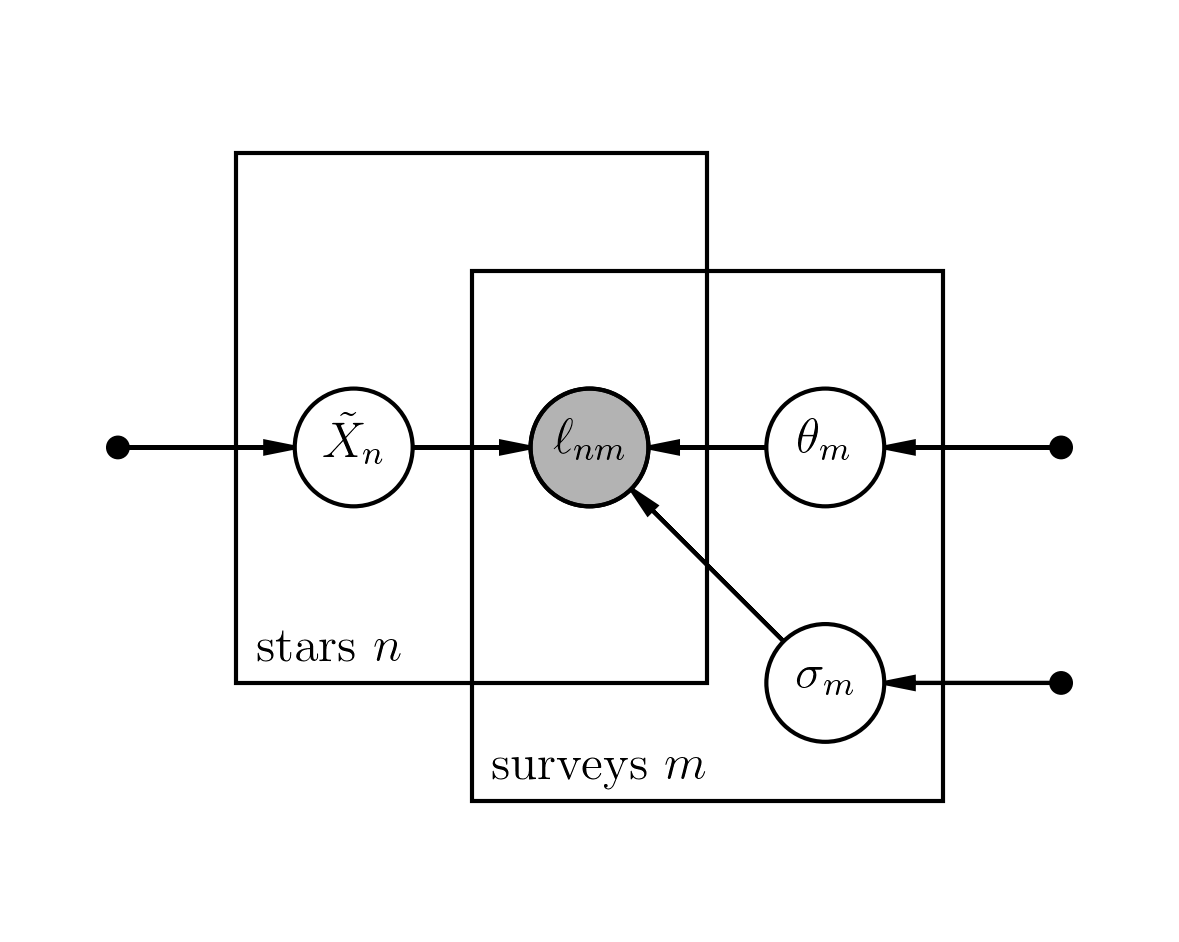
\includegraphics[width=0.5\textwidth]{figures/pgm.png}
    \caption{A graphical representation of the latent variable model we adopt.}
    \label{fig:pgm}
\end{figure}


\acknowledgements

It is a pleasure to thank
	Dan Foreman-Mackey
for useful conversations.
This work was partly supported through the Australian Research Council 
through Discovery Grant DP160100637.


\software{
	\package{Astropy} \citep{astropy},
    \package{IPython} \citep{ipython},
    \package{matplotlib} \citep{mpl},
    \package{numpy} \citep{numpy},
    \package{scipy} \citep{scipy},
    \package{Stan} \citep{stan},
    \package{Daft} % http://daft-pgm.org/
    %tensorflow
}    

\bibliographystyle{aasjournal}
\bibliography{uberchemical}



\end{document}
